%auto-ignore
 
\definecolor{light-gray}{gray}{0.6}
\begin{figure}[H]
  \centering
  %\begin{subfigure}[b]{0.15\textwidth}
    \begin{tikzpicture}[scale=1.0,auto,swap]

    % the two brain figures on top
    \node (upper_brain) at (0,1.5) { \includegraphics*[scale=\scaleBrainImg,trim=0 0 240 0]{\snapLocationEAR/stage_1.eps}};
    \node (lower_brain) at (0,-1.5) { \includegraphics*[scale=\scaleBrainImg,trim=240 0 0 0]{\snapLocationEAR/stage_1.eps}};
    \node[above=0cm of upper_brain] (stage) {Stage 1};
    % the balls
    
    \end{tikzpicture}
  %\end{subfigure}
  % next subfigure
  \hspace{-1.5em}
  ~
  %\begin{subfigure}[b]{0.15\textwidth}
    \begin{tikzpicture}[scale=1.0,auto,swap]

    % the two brain figures on top
    \node (upper_brain) at (0,1.5) { \includegraphics*[scale=\scaleBrainImg,trim=0 0 240 0]{\snapLocationEAR/stage_2.eps}};
    \node (lower_brain) at (0,-1.5) { \includegraphics*[scale=\scaleBrainImg,trim=240 0 0 0]{\snapLocationEAR/stage_2.eps}};
    \node[above=0cm of upper_brain] (stage) {Stage 2};
    % the balls
    
    \end{tikzpicture}
  %\end{subfigure}
  % next subfigure
  \hspace{-1.5em}
  ~
  %\begin{subfigure}[b]{0.15\textwidth}
    \begin{tikzpicture}[scale=1.0,auto,swap]

    % the two brain figures on top
    \node (upper_brain) at (0,1.5) { \includegraphics*[scale=\scaleBrainImg,trim=0 0 240 0]{\snapLocationEAR/stage_3.eps}};
    \node (lower_brain) at (0,-1.5) { \includegraphics*[scale=\scaleBrainImg,trim=240 0 0 0]{\snapLocationEAR/stage_3.eps}};
    \node[above=0cm of upper_brain] (stage) {Stage 3};
    % the balls
    
    \end{tikzpicture}
  %\end{subfigure}
  % next subfigure
  \hspace{-1.5em}
  ~
  %\begin{subfigure}[b]{0.15\textwidth}
    \begin{tikzpicture}[scale=1.0,auto,swap]

    % the two brain figures on top
    \node (upper_brain) at (0,1.5) { \includegraphics*[scale=\scaleBrainImg,trim=0 0 240 0]{\snapLocationEAR/stage_4.eps}};
    \node (lower_brain) at (0,-1.5) { \includegraphics*[scale=\scaleBrainImg,trim=240 0 0 0]{\snapLocationEAR/stage_4.eps}};
    \node[above=0cm of upper_brain] (stage) {Stage 4};
    % the balls
    
    \end{tikzpicture}
  %\end{subfigure}
  % next subfigure
  \hspace{-1.5em}
  ~
  %\begin{subfigure}[b]{0.15\textwidth}
    \begin{tikzpicture}[scale=1.0,auto,swap]

    % the two brain figures on top
    \node (upper_brain) at (0,1.5) { \includegraphics*[scale=\scaleBrainImg,trim=0 0 240 0]{\snapLocationEAR/stage_5.eps}};
    \node (lower_brain) at (0,-1.5) { \includegraphics*[scale=\scaleBrainImg,trim=240 0 0 0]{\snapLocationEAR/stage_5.eps}};
    \node[above=0cm of upper_brain] (stage) {Stage 5};
    % the balls
    
    \end{tikzpicture}
  %\end{subfigure}
  % next subfigure
  \hspace{-1.5em}
  ~
  %\begin{subfigure}[b]{0.15\textwidth}
    \begin{tikzpicture}[scale=1.0,auto,swap]

    % the two brain figures on top
    \node (upper_brain) at (0,1.5) { \includegraphics*[scale=\scaleBrainImg,trim=0 0 240 0]{\snapLocationEAR/stage_6.eps}};
    \node (lower_brain) at (0,-1.5) { \includegraphics*[scale=\scaleBrainImg,trim=240 0 0 0]{\snapLocationEAR/stage_6.eps}};
    \node[above=0cm of upper_brain] (stage) {Stage 6};
    % the balls
    
    \end{tikzpicture}
  %\end{subfigure}
  % next subfigure
  \hspace{-1.5em}
  ~
  %\begin{subfigure}[b]{0.15\textwidth}
    \begin{tikzpicture}[scale=1.0,auto,swap]

    % the two brain figures on top
    \node (upper_brain) at (0,1.5) { \includegraphics*[scale=\scaleBrainImg,trim=0 0 240 0]{\snapLocationEAR/stage_7.eps}};
    \node (lower_brain) at (0,-1.5) { \includegraphics*[scale=\scaleBrainImg,trim=240 0 0 0]{\snapLocationEAR/stage_7.eps}};
    \node[above=0cm of upper_brain] (stage) {Stage 7};
    % the balls
    
    \end{tikzpicture}
  %\end{subfigure}
  % next subfigure
  \hspace{-1.5em}
  ~
  %\begin{subfigure}[b]{0.15\textwidth}
    \begin{tikzpicture}[scale=1.0,auto,swap]

    % the two brain figures on top
    \node (upper_brain) at (0,1.5) { \includegraphics*[scale=\scaleBrainImg,trim=0 0 240 0]{\snapLocationEAR/stage_8.eps}};
    \node (lower_brain) at (0,-1.5) { \includegraphics*[scale=\scaleBrainImg,trim=240 0 0 0]{\snapLocationEAR/stage_8.eps}};
    \node[above=0cm of upper_brain] (stage) {Stage 8};
    % the balls
    
    \end{tikzpicture}
  %\end{subfigure}
  % next subfigure
  \hspace{-1.5em}
  ~
  %\begin{subfigure}[b]{0.15\textwidth}
    \begin{tikzpicture}[scale=1.0,auto,swap]

    % the two brain figures on top
    \node (upper_brain) at (0,1.5) { \includegraphics*[scale=\scaleBrainImg,trim=0 0 240 0]{\snapLocationEAR/stage_9.eps}};
    \node (lower_brain) at (0,-1.5) { \includegraphics*[scale=\scaleBrainImg,trim=240 0 0 0]{\snapLocationEAR/stage_9.eps}};
    \node[above=0cm of upper_brain] (stage) {Stage 9};
    % the balls
    
    \end{tikzpicture}
  %\end{subfigure}
  % next subfigure
  \hspace{-1.5em}
  ~
  \hspace{1em}
  % the red-to-yellow gradient on the right
  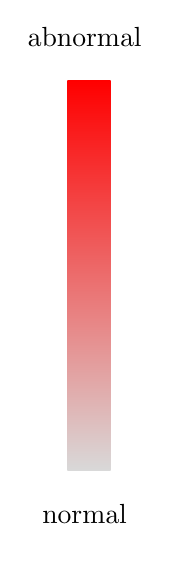
\begin{tikzpicture}[scale=1.1,auto,swap]
    \shade[top color=red,bottom color=gray!30] (0,1.5) rectangle (0.5,6);
    \node[inner sep=0] (corr_text) at (0.2,6.5) {abnormal};
    \node[inner sep=0] (corr_text) at (0.2,1) {normal};
    \node[inner sep=0] (corr_text) at (0.2,0.5) {};
  \end{tikzpicture}
  \captionSnapEBMEAR
\end{figure}



